\chapter{No-name yet}

\newpage

\section{Query taxonomy and re-usability formalization}

This section presents the description and formalization of the different types of queries which \textit{(i)} can be processed by our integration approach; and \textit{(ii)} can be compared to previous integration requests in order to take advantage from previous integration plans. The query definition is introduced below.

\begin{definition}
A query is defined as a $n$-tuple:
%
\begin{center}
$Q := \langle s, t, A, R, S, C, w  \rangle$
\end{center}
%
where: $A$ is a set of abstract services defining the query $Q$;
$R$ is a set of user preferences that can be defined over the data services or the entire query;
$S$ is a set of data services that were selected satisfying the restrictions defined by $R$ to potentially rewrite the query $Q$;
$C$ is a set of compositions that were produced using the data services in $S$ and satisfying the restrictions defined by $R$ that potentially can answer the query $Q$; and
$w$ is the composition that were selected and executed to answer the query $Q$. 
\end{definition}

The query taxonomy proposed below is defined according to the type of relation that can be established between two queries. 
Queries are classified in four groups: 
\begin{itemize}
\item \textit{Group 1:} The data denoted by the answer of $Q_{1}$ is the same data expected by the answer of $Q_{2}$. For example, $Q_{1}$ and $Q_{2}$ retrieve patients that were infected by pneumonia.
\item \textit{Group 2:} The data denoted by the answer of $Q_{1}$ is a subset of the data denoted by the answer of $Q_{2}$. For example, $Q_{2}$ retrieves patients that were infected by pneumonia and $Q_{1}$ retrieves patients that were infected by pneumonia and treated by the doctor Lucas.
\item \textit{Group 3:} The data denoted by the answer of $Q_{1}$ is a superset of the data denoted by the answer of $Q_{2}$. For example, $Q_{2}$ retrieves patients that were infected by pneumonia and treated by the doctor Lucas, and $Q_{1}$ retrieves patients that were infected by pneumonia.
\item \textit{Group 4:} The data denoted by the answer of $Q_{1}$ is different of the data denoted by the answer of $Q_{2}$. For example, $Q_{2}$ retrieves patients that were infected by pneumonia and treated by the doctor Lucas, and $Q_{1}$ retrieves patients that were infected by pneumonia with admission in the hospital Edouard Herriot.
\end{itemize}

To understand the different types of query, basic concepts regarding \textit{(i)} user requirements, \textit{(ii)} requirements domain, \textit{(iii)} requirements evaluation and \textit{(iv)} comparable requirements should be introduced:

\begin{definition}
An user requirement $r$ is in the form $x \otimes c$, where $x$ is an identifier; $c$ is a constant; and $\otimes \in\lbrace \geq, \leq, =, \neq, <, >\rbrace$. 
%
The user requirement $r$ could concern \textit{(i)} the entire \textsl{query}, in this case noted as $r_{Q}$; or \textit{(ii)} a single service, noted as $r_{S}$. For instance, the total response time is obtained by adding the response time of each service involved in the composition.
\end{definition}

\begin{definition}
A requirement domain is a set of possible values which can be assumed by an user requirement $r$, represented by $Dom(r)$. 
For instance, a requirement domain ``response time'' includes the possible values associated to the response time user requirement. 
Each user requirement $r_{i}$ has its own requirement domain $D_{i}$. 
\end{definition}

\begin{definition}
The evaluation of an user requirement $r$, indicated by $eval(r)$, returns a set of values $\lbrace v_{1},..,v_{i} \rbrace$ that can be assigned to $r$ such that $\lbrace v_{1},..,v_{i} \rbrace \subset Dom(r)$.
\end{definition}

\begin{definition}
Given two user requirements $r_{1}$ and $r_{2}$, both can be comparable, denoted by $r_{1} \perp r_{2}$, if and only if:  $Dom(r_{1}) = Dom(r_{2})$.
\end{definition}

The thirteen types of queries included in the taxonomy described in the following sections are organized according to their groups.

\subsection{Queries that can potentially be completely reusable}

There are two types of queries belonging to this group. Given a previous query $Q_{1}$ stored in the query history and an incoming query $Q_{2}$, the types are: \textit{(i)} $Q_{1}$ and $Q_{2}$ are completely equivalents (the simplest case); and \textit{(ii)} $Q_{1}$ and $Q_{2}$ comprehend the same abstract services but $Q_{2}$ specifies user requirements less restrict than $Q_{1}$. The characteristics of these queries are described below:

\begin{enumerate}[a)]
\item \textit{Query type 1:} the \textit{first} type is the simplest case. The figure~\ref{fig:qt1} illustrates the manner this query is represented. Given a previous query $Q_{1}$ and an incoming query $Q_{2}$, $Q_{1}$ is equivalent to $Q_{2}$ when: \textit{(1)} both queries expect the same data as answer, which means they cover the same abstract services (Figure~\ref{fig:qt1} - Data point of view). In this sense, the set of abstract service of $Q_{1}$, denoted as $Q_{1}.A$, is equals to the set of abstract services of $Q_{2}$, denoted as $Q_{2}.A$.
%
\begin{center}
$Q_{1}.A = Q_{2}.A$
\end{center}
%
\textit{(2)} For each user requirement $r_{i}$ in $Q_{1}.R$, there is a user requirement $r_{j}$ in $Q_{2}.R$ such that the evaluation of $r_{i}$ is equal to the evaluation of $r_{j}$. 
Consequently, the score of $Q_{1}.R$ is equals to the score of $Q_{2}.R$. The \textit{query type 1} and the equivalence between requirements are formally defined below.
\end{enumerate}

\begin{figure}[!htbp]
\center
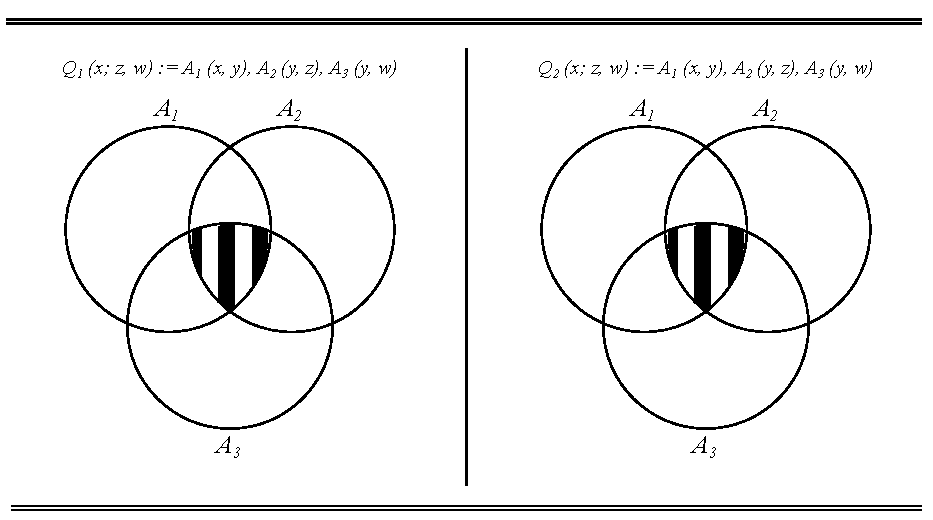
\includegraphics[scale=0.7]{images/QT2-ABSTRACT-SERVICES.pdf}
\caption{Query type 2 representation.}
\label{fig:qt2}
\end{figure}

\begin{definition}\label{def:reqeq}
A set of user requirements $R_{1}$ is equivalent to a set of \textsl{user requirements} $R_{2}$, represented by $R_{1} \equiv R_{2}$, if and only if: $\forall r_{i} \in R_{1}, \ \exists r_{j} \in R_{2} \ \vert \ eval (r_{i}) = eval(r_{j}) \ and \ \vert R_{1} \vert = \vert R_{2} \vert$.
\end{definition}

\begin{definition}\label{def:qt1}
Query Type 1 -- a query $Q_{1}$ is equivalent to a query $Q_{2}$, if and only if: $Q_{1}.A = Q_{2}.A$ and $Q_{1}.R_{1} \equiv Q_{2}.R_{2}$.
\end{definition}

From the re-usability point of view, everything from $Q_{1}$ could be reused to answer $Q_{2}$. All data services filtered to the query $Q_{1}$, denoted $Q_{1}.S$, potentially could be reused in the query $Q_{2}$, excepting the ones that are not online in the exact moment. 

\begin{figure}[!htbp]
\center
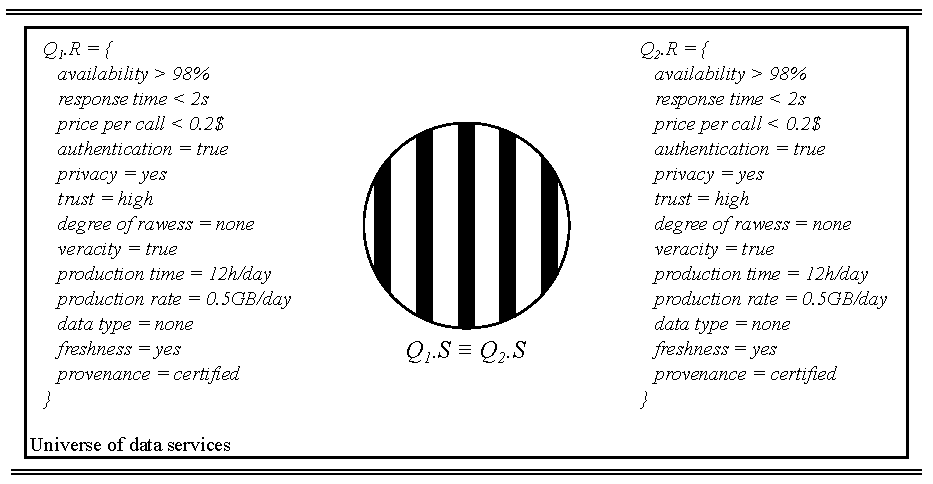
\includegraphics[scale=0.7]{images/QT1-DATA-SERVICES.pdf}
\caption{Query type 1 representation.}
\label{fig:qt1}
\end{figure}

The set of compositions produced to the query $Q_{1}$, denoted as $Q_{1}.C$, potentially could be used to answer the query $Q_{2}$, excepting the ones using offline data services. Following, the reusability function for data services, rewritings and queries are presented. 

\begin{figure}[!h]
\center
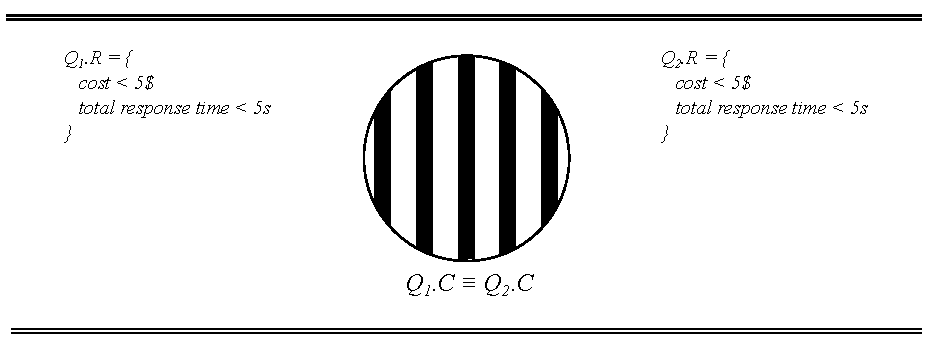
\includegraphics[scale=0.7]{images/QT1-COMPOSITIONS.pdf}
\caption{Query type 1 - relation between composition sets.}
\label{fig:qt1-c}
\end{figure}

The service reusability function -- denoted as $reuse\_services(q_{1},\ q_{2})$ where $q_{1}$ is a stored query and $q_{2}$ an incoming query -- returns a set of reusable data services for $q_{2}$ based on the data services of $q_{1}$.

\begin{definition}\label{def:rsqt1}
The service reusability function $reuse\_services(q_{1},\ q_{2})$ -- for queries of group 1 -- returns a set of data services $S_{o}$, which are online in this exact moment in the data services of $q_{1}$. 
\begin{center}
$ S_{o} \leftarrow S_{o} \ \cup \ \lbrace ds_{i} \rbrace\ such\ that\ \lbrace \forall ds_{i} \in q_{1}.S \ \vert \ ds_{i} \ is \ online\rbrace$.
\end{center}
\end{definition}

The rewritings reusability function -- denoted as $reuse\_rewritings(q_{1},\ q_{2})$ where $q_{1}$ is a stored query and $q_{2}$ an incoming query -- returns a set of reusable compositions to answer $q_{2}$ based on the data services and compositions of $q_{1}$.

\begin{definition}\label{def:rrqt1}
The rewritings reuse function $\mathbf{reuse\_rewritings(q_{1},\ q_{2})}$ returns a set of rewritings $C_{o}$, which uses the data services $S_{o}$ returned by $reuse\_services(q_{1},\ q_{2})$. 
\begin{center}
$C_{o} \leftarrow C_{o} \ \cup \ \lbrace c_{i} \rbrace\ \vert\ \lbrace \forall c_{i} \in q_{1}.C,\ \exists ds_{j} \in c_{i},\ \nexists ds_{k} \in c_{i} \ \vert \
   ds_{j} \in S_{o} \ and \ ds_{k} \notin S_{o} \rbrace$.
\end{center}
\end{definition}

\begin{enumerate}[b)]
\item \textit{Query type 2} comprehends a query case including less restrict user requirements.  
This type of query is a general case of \textit{query type 1} as introduced in the figure~\ref{fig:qt2}.
Given a previous query $Q_{1}$ and an incoming query $Q_{2}$, $Q_{2}$ is a subset case of $Q_{1}$ when: \textit{(1)} both queries expect the same data as answer, which means they cover the same abstract services. 
For example, in the figure~\ref{fig:qt2} (Data point of view), it possible to note that both queries includes the abstract services $A_{1}$, $A_{2}$ and $A_{3}$ in their definition.
In this sense, the set of abstract service of $Q_{1}$, denoted as $Q_{1}.A$, is equals to the set of abstract services of $Q_{2}$, denoted as $Q_{2}.A$.  
%
\begin{center}
$Q_{1}.A = Q_{2}.A$
\end{center}
%
\textit{(2)} There exists at least one user requirement $r_{i}$ in $Q_{2}.R$ and $r_{j}$ in $Q_{1}.R$ such that the evaluation of $r_{i}$ contains the evaluation of $r_{j}$. 
\textit{(3)} There not exists a user requirement $r_{k}$ in $Q_{2}.R$ such that the evaluation of $r_{k}$ is contained in the evaluation of $r_{j}$.
Consequently, the score of $Q_{1}.R$ is higher than the score of $Q_{2}.R$. 
The \textit{query type 2} and the less restrict user requirements are formally defined below.
\end{enumerate}

\begin{definition}
Given a set of user requirements $R_{1}$ and $R_{2}$, $R_{1}$ is less restrict than $R_{2}$, represented by $R_{1} \ \lhd \ R_{2}$, if and only if: 
$\forall r_{i} \in R_{1}, \ \exists r_{j} \in R_{2}, \ \nexists r_{k} \in R_{2} \ \ \vert \ eval (r_{i}) \supset eval(r_{j}) \ and \ eval (r_{i}) \subset eval(r_{k}) \ and \ \vert R_{1} \vert = \vert R_{2} \vert$.
\end{definition}

\begin{definition}\label{def:qt1}
Query Type 2 -- a query $Q_{2}$ is a subset case of a query $Q_{1}$, if and only if: $Q_{1}.A = Q_{2}.A$ and $Q_{2}.R \lhd Q_{1}.R$.
\end{definition}

Once queries of \textit{type 2} are general cases of queries of \textit{type 1}, $Q_{2}$ could profit from the entire data (data services and compositions) collected/stored to answer $Q_{1}$. 
The set of data services selected to $Q_{1}$ ($Q_{1}.S$) -- respecting the user requirements specified in $Q_{1}$ -- is a potential subset of the data services selected to $Q_{2}$ ($Q_{2}.S$).
In other words, $Q_{1}.S$ is contained in the set $Q_{2}.S$ (see figure~\ref{fig:qt2-ds}).
Although $Q_{2}.S$ could accept other data services which are not in $Q_{1}.S$ (if the rewriting process was launched from the beginning), all data services from $Q_{1}.S$ are reusable in $Q_{2}.S$ excepting the services offline in the exact moment. 
The service reusability function for queries \textit{type 2} is the same defined for the queries \textit{type 1} (see definition~\ref{def:rsqt1}).

\begin{figure}[!h]
\center
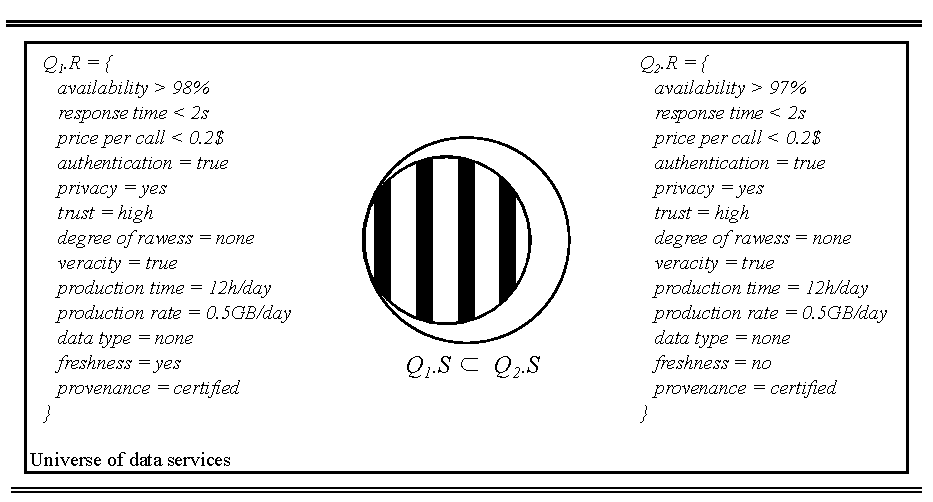
\includegraphics[scale=0.7]{images/QT2-DATA-SERVICES.pdf}
\caption{Query type 2 - relation between sets of data services.}
\label{fig:qt2-ds}
\end{figure}

The set of compositions produced to the query $Q_{1}$ ($Q_{1}.C$) is a potential subset of the compositions to answer the query $Q_{2}$ even if the user requirements of $Q_{2}$ ($Q_{2}.R$) are less restrict than the requirements of $Q_{1}$ ($Q_{1}.R$). 
This means $Q_{1}.C$ is contained in $Q_{2}.C$ (see figure~\ref{fig:qt2-c}).
Although $Q_{2}$ could be answered by other compositions which are not in $Q_{1}.C$ (if the rewriting process was launched from the beginning), all compositions from $Q_{1}.C$ are reusable in $Q_{2}.C$ excepting those that uses data services offline in the exact moment. 
The rewritings reusability function for queries of \textit{type 2} is the same defined for queries \textit{type 1} (see definition~\ref{def:rrqt1}). 

\begin{figure}[!h]
\center
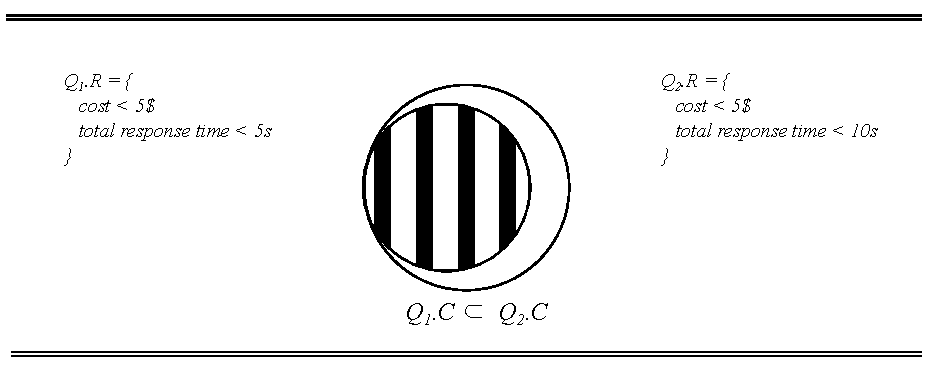
\includegraphics[scale=0.7]{images/QT2-COMPOSITIONS.pdf}
\caption{Query type 2 - relation between sets of data services.}
\label{fig:qt2-c}
\end{figure}

Finally, the query reusability function -- denoted as $\mathbf{reuse\_query(q_{1}, \ q_{2})}$ where $q_{1}$ is a stored query and $q_{2}$ a incoming query -- provides the information concerning the data services and compositions that can be used to answer the user request by reusing results from $q_{1}$ in $q_{2}$. 

\begin{definition}
The query reusability function $\mathbf{reuse\_query(q_{1}, \ q_{2})}$ returns $q_{2}$ such that $q_{2}.S \leftarrow reuse\_services(q_{1}, q_{2}) \ and \ q_{2}.C \leftarrow reuse\_rewritings(q_{1}, q_{2})$.
\end{definition}

\textcolor{red}{Atualizar funcoes antes de passar para o outro grupo.}

\textcolor{red}{daqui para baixo sera o outro grupo}

\subsection{Group 2}

\begin{enumerate}[a)]
\item Query equivalent with user requirements more restrict
\end{enumerate}

\begin{definition}
$Q_{1}.A = Q_{2}.A$
\end{definition}

\begin{definition}
Definir servico concreto: 
\begin{center}
$ds := \langle A, R  \rangle$
\end{center}
\end{definition}

\begin{definition}
Definir QoS aspects of the service respect user requirements, denoted ds satisfies R: 
\begin{center}
$\forall r_{i} \in ds.R, \ \exists r_{j} \in R_{q} \ \vert \ eval (r_{i}) = eval(r_{j}) \ or \ eval (r_{i}) \subset eval(r_{j})$.
\end{center}
\end{definition}

\begin{definition}\label{def:??}
%The service reusability function $reuse\_services(q_{1},\ q_{2})$ -- for queries of group 1 -- returns a set of data services $S_{o}$, which are online in this exact moment in the data services of $q_{1}$. 
\textbf{RS-2}
\begin{center}
$ S_{o} \leftarrow S_{o} \ \cup \ \lbrace ds_{i} \rbrace\ such\ that\ \lbrace \forall ds_{i} \in q_{1}.S \ \vert \ ds_{i} \ is \ online\ and\ ds_{i}\ satisfies\ q_{2}.R \rbrace$.
\end{center}
reuse rewriting: \textbf{RR-1}
\end{definition}

\begin{enumerate}[b)]
\item Query equivalent with user requirements more and less restrict. Definicoes iguais ao anterior.
\end{enumerate}

\subsection{Group 3}

\begin{enumerate}[a)]
\item Query q2 is a subset of q1 with equivalent user requirements
\end{enumerate}

\begin{definition}
$Q_{1}.A \subset Q_{2}.A$
\end{definition}

\begin{definition}\label{def:??}
%The service reusability function $reuse\_services(q_{1},\ q_{2})$ -- for queries of group 1 -- returns a set of data services $S_{o}$, which are online in this exact moment in the data services of $q_{1}$. 
Igual ao query type 1. O reuse rewritings tb.
\begin{center}
$ S_{o} \leftarrow S_{o} \ \cup \ \lbrace ds_{i} \rbrace\ such\ that\ \lbrace \forall ds_{i} \in q_{1}.S \ \vert \ ds_{i} \ is \ online\ \rbrace$.
\end{center}
\end{definition}

% RQ-2
\begin{definition}
Given two queries $Q_{1}$ and $Q_{1}$ as follows:
\begin{center}
$Q_{1} = \langle s,\ t,\ A,\ R,\ S,\ C,\ w \rangle$ \\
$Q_{2} = \langle s,\ t,\ A,\ R,\ S?,\ C?,\ w? \rangle$
\end{center}
Where query $Q_{2}$ contains undefined sets of data services ($Q_{2}.S?$) and compositions ($Q_{2}.C?$), and the composition ($Q_{2}.w?$) selected to answer the request.
The query reusability function of $Q_{2}$ based on $Q_{1}$, denoted as $reuse\_query(Q_{1},\ Q_{2})$, completes and returns $Q_{2}$ such that:
\begin{center}
$ Q_{2}.S \leftarrow S_{i}\ \cup\ S_{Q_{2}-Q_{1}} $
\end{center}
Where $ S_{i}$ is a set of reusable data services obtained from $Q_{1}.S$ and $S_{Q_{2}-Q_{1}}$ is a set of data services selected by the algorithm X:
\begin{center}
$S_{i} \leftarrow reuse\_service (Q_{1},\ Q_{2})$ \\
$S_{Q_{2}-Q_{1}} \leftarrow algorithm\_X (Q_{1},\ Q_{2})$
\end{center}
This algorithm is responsible (i) to identify and (ii) to select data services that cover the abstract services in the set $Q_{2}.A - Q_{1}.A$. In other words, it selects services that are necessary to complete $Q_{1}$ compositions to satisfy $Q_{2}$.

The set of compositions of $Q_{2}$ is obtained by invoking the algorithm Y.
\begin{center}
$Q_{2}.C \leftarrow algorithm\_Y (C_{0}, S_{Q_{2}-Q_{1}}, Q_{2})$
\end{center}
This algorithm is a simple and reduced rewriting step responsible to improve each composition in $Q_{1}.C$ adding the absent services to satisfy $Q_{2}$. 
The algorithm expects three inputs (i) the set of reusable compositions $C_{0}$ from $Q_{1}$ obtained from the reuse rewriting function: 
\begin{center}
$ C_{0} \leftarrow reuse\_rewritings (Q_{1},\ Q_{2})$
\end{center}
ii) the set of services to complete the compositions $S_{Q_{2}-Q_{1}}$; and (iii) the query  $Q_{2}$.
%\begin{flushleft}
%$ S_{0} \leftarrow reuse\_service (q_{1}, q_{2})$. \\
%$ S_{1} \leftarrow algorithm\_X (q_{1}, q_{2})$. \\
%$ C_{0} \leftarrow reuse\_rewritings (q_{1}, q_{2})$. \\
%$ C_{1} \leftarrow algorithm\_Y (C_{0}, S_{1}, q_{2})$. \\
%$ q_{2}.S \leftarrow S_{0} \cup S_{1}\ and\ q_{2}.C \leftarrow C_{1}$.
%\end{flushleft}
Finally, the composition $Q_{2}.w$ selected to answer $Q_{2}$ is the one with the highest score among the compositions in the set $Q_{2}.C$. 
The query $Q_{2}$ is now complete.
\end{definition}

\begin{enumerate}[b)]
\item Query q2 is a subset of q1 with user requirements less restrict
\end{enumerate}

\begin{definition}
Tudo igual ao anterior...
\end{definition}

\subsection{Group 4}

\begin{enumerate}[a)]
\item Query q2 is a subset of q1 with user requirements more restrict
\item Query q2 is a subset of q1 with user requirements more/less restrict
\end{enumerate}

\begin{definition}
\textbf{RS-2} \textbf{RR-1} and \textbf{RQ-2}
\end{definition}

\subsection{Group 5}
\begin{enumerate}[a)]
\item Query q2 is a superset of q1 with user requirements equivalents
\item Query q2 is a superset of q1 with user requirements less restrict
\end{enumerate}

\begin{definition}
Data service ds covers the query q: 
\begin{center}
$ \forall a_{i} \in ds.A,\ \nexists a_{j} \in ds.A \ \vert \ a_{i} \in q.A\ and\ a_{j} \notin q.A$
\end{center}
\end{definition}

\begin{definition}
\textbf{RS-3}:
\begin{flushleft}
$ S_{o} \leftarrow S_{o} \ \cup \ \lbrace ds_{i} \rbrace\  st.\ \lbrace \forall ds_{i} \in q_{1}.S\ \vert \ ds_{i} \ is \ online\ and\ ds_{i}\ covers\ q_{2} \rbrace$. \\
\end{flushleft}
\end{definition}

\textbf{RR1 igual..}

\begin{definition}
\textbf{RQ-3}:
\begin{flushleft}
$ S_{0} \leftarrow reuse\_service (q_{1}, q_{2})$. \\
$ C_{0} \leftarrow reuse\_rewritings (q_{1}, q_{2})$. \\
$ C_{1} \leftarrow algorithm\_Z (C_{0}, q_{2})$. \\
$ q_{2}.S \leftarrow S_{0} and\ q_{2}.C \leftarrow C_{1}$.
\end{flushleft}
\end{definition}

\subsection{Group 6}
\begin{enumerate}[a)]
\item Query q2 is a superset of q1 with user requirements more restrict
\item Query q2 is a superset of q1 with user requirements more/less restrict
\end{enumerate}

\begin{definition}
\textbf{RS-4}:
\begin{flushleft}
$ S_{o} \leftarrow S_{o} \ \cup \ \lbrace ds_{i} \rbrace\  st.\ \lbrace \forall ds_{i} \in q_{1}.S\ \vert \ ds_{i} \ is \ online\ and\ ds_{i}\ covers\ q_{2}\ and\ \newline ds_{i}\ satisfies\ q_{2}.R\ \rbrace$. \\
\end{flushleft}

\textbf{RR1 and RQ-3}
\end{definition}


\subsection{Group 7}
\begin{enumerate}[a)]
\item Query q2 is different from q1 but both have abstract services in common

\begin{definition}
$ \forall a_{i} \in q_{1}.A,\ \exists a_{j} \in  q_{1}.A,\ \exists a_{k} \in  q_{2}.A\ \vert \newline  
a_{j} \subset  q_{2}.A\ and\ 
a_{j} \subsetneq  q_{2}.A\ and\
a_{k} \subsetneq  q_{1}.A \rbrace$. \\
$n(Q_{1}.A \cap Q_{2}.A) > 1$ \\
caso contrario eh melhor reescrever
\end{definition}
\end{enumerate}

\begin{definition}
\textbf{RS-4} and \textbf{RR-1} iguais....
\end{definition}

\begin{definition}
\textbf{RQ-4}:
\begin{flushleft}
$ S_{0} \leftarrow reuse\_service (q_{1}, q_{2})$. \\
$ S_{1} \leftarrow algorithm\_X (q_{1}, q_{2})$. \\
$ C_{0} \leftarrow reuse\_rewritings (q_{1}, q_{2})$. \\
$ C_{1} \leftarrow algorithm\_w (C_{0}, S_{1}, q_{2})$. \\
$ q_{2}.S \leftarrow S_{0} \cup S_{1}\ and\ q_{2}.C \leftarrow C_{1}$.
\end{flushleft}
\end{definition}

\textbf{A case outside of this taxonomy requires a full rewriting process.}

\subsubsection{Query type 2: $Q_{2}$ is a subset of $Q_{1}$}

The \textit{second} type deals with \textit{query subsets} due to more restrict user requirements. Given two queries $Q_{1}$ and $Q_{2}$, $Q_{2}$ is a subset of $Q_{1}$ when:
%
\begin{enumerate}[a)]
\item They expect the same data as answer, which means they cover the same abstract services. 
For instance, the set of abstract service of $Q_{1}$, denoted as $Q_{1}.A$, is equals to the set of abstract services of $Q_{2}$, denoted as $Q_{2}.A$.
%
\begin{center}
$Q_{1}.A = Q_{2}.A$
\end{center}
%
\item For all user requirement $r_{i}$ in $Q_{2}.R$, there is at least one $r_{j}$ in $Q_{1}.R$ such that the evaluation of $r_{i}$ is contained in the evaluation of $r_{j}$. 
For all $r_{k}$ in $Q_{2}.R$, there is no $r_{l}$ in $Q_{1}.R$ such that the evaluation of $r_{l}$ is contained in the evaluation of $r_{k}$. 
Consequently, the score of $Q_{1}.R$ is lower than the score of $Q_{2}.R$. The definition of more restrict requirements is presented below.
\end{enumerate}

\begin{definition}\label{def:reqmore}
Given a set of \textsl{user requirements} $R_{1}$ and $R_{2}$, $R_{1}$ is more restrict than $R_{2}$, represented by $R_{1} \ \rhd \ R_{2}$, if and only if: $\forall r_{i} \in R_{1}, \ \exists r_{j} \in R_{2}, \ \nexists r_{k} \in R_{2} \ \vert \ eval (r_{i}) \subset eval(r_{j}) \ and \ eval (r_{k}) \subset eval(r_{i}) \ and \ \vert R_{1} \vert = \vert R_{2} \vert$.
\end{definition}

From the re-usability point of view, a subset of the data services filtered to the query $Q_{1}$ which are \textit{online} in the moment, $online(Q_{1}.S)$, could be reused in the query $Q_{2}$. This fact occurs due to the more restrict requirements imposed by $Q_{2}$.
With respect to the compositions, a subset of the rewritings produced to the query $Q_{1}$ could also be used to answer the query $Q_{2}$. These rewritings should use the data services in $online(Q_{1}.S)$, denoted as $available(Q_{1}.C)$, and respect the more restrict requirements defined in $Q_{2}$. 
The query type 2 definition is presented below.

\begin{definition}\label{def:qt2}
Query Type 3 -- a query $Q_{1}$ is a subset of a query $Q_{2}$, if and only if: $Q_{1}.A = Q_{2}.A$ and $Q_{1}.R_{1} \rhd Q_{2}.R_{2}$
\end{definition}


\begin{definition}\label{def:reqmoreless}
Given a set of  requirements $R_{1}$ and $R_{2}$, $R_{1}$ contains mixed types of requirements compared to $R_{2}$, represented by $R_{1} \ \neq \ R_{2}$, if and only if: $\forall r_{i} \in R_{1}, \ \exists r_{j} \in R_{2}, \ \exists r_{k} \in R_{2} \ \vert \ eval (r_{i}) \subset eval(r_{j}) \ and \ eval (r_{k}) \subset eval(r_{i}) \ and \ \vert R_{1} \vert = \vert R_{2} \vert$.
\end{definition}

\begin{definition}\label{def:qt2}
Query Type 4 -- a query $Q_{2}$ is a subset of a query $Q_{1}$, if and only if: $Q_{1}.A = Q_{2}.A$ and $Q_{1}.R_{1} \neq Q_{2}.R_{2}$
\end{definition}

\begin{definition}\label{def:qt2}
Query Type 5 -- a query $Q_{2}$ is a superset of a query $Q_{1}$, if and only if: $Q_{1}.A \subset Q_{2}.A$ and $Q_{1}.R_{1} \equiv Q_{2}.R_{2}$
\end{definition}

\begin{definition}\label{def:qt2}
Query Type 6 -- a query $Q_{2}$ is a superset of a query $Q_{1}$, if and only if: $Q_{1}.A \subset Q_{2}.A$ and $Q_{2}.R \triangleleft Q_{1}.R$
\end{definition}

\begin{definition}\label{def:qt2}
Query Type 7 -- a query $Q_{2}$ is a superset of a query $Q_{1}$, if and only if: $Q_{1}.A \subset Q_{2}.A$ and $Q_{2}.R \triangleright Q_{1}.R$
\end{definition}

\begin{definition}\label{def:qt2}
Query Type 8 -- a query $Q_{2}$ is a superset of a query $Q_{1}$, if and only if: $Q_{1}.A \subset Q_{2}.A$ and $Q_{2}.R \neq Q_{1}.R$
\end{definition}

\begin{definition}\label{def:qt2}
Query Type 9 -- a query $Q_{2}$ is a subset of a query $Q_{1}$, if and only if: $Q_{1}.A \supset Q_{2}.A$ and $Q_{2}.R \equiv Q_{1}.R$
\end{definition}

\begin{definition}\label{def:qt2}
Query Type 10 -- a query $Q_{2}$ is a subset of a query $Q_{1}$, if and only if: $Q_{1}.A \supset Q_{2}.A$ and $Q_{2}.R \triangleleft Q_{1}.R$
\end{definition}

\begin{definition}\label{def:qt2}
Query Type 11 -- a query $Q_{2}$ is a subset of a query $Q_{1}$, if and only if: $Q_{1}.A \supset Q_{2}.A$ and $Q_{2}.R \triangleright Q_{1}.R$
\end{definition}

\begin{definition}\label{def:qt2}
Query Type 12 -- a query $Q_{2}$ is a subset of a query $Q_{1}$, if and only if: $Q_{1}.A \supset Q_{2}.A$ and $Q_{2}.R \neq Q_{1}.R$
\end{definition}

\begin{definition}\label{def:qt2}
Query Type 13 -- a query $Q_{2}$ is different of a query $Q_{1}$, but sharing abstract services, if and only if: $Q_{1}.A \neq Q_{2}.A$ and $n(Q_{1}.A \cap Q_{2}.A) > 1$.
\end{definition}